\section{Technical Overview}
\label{sec:katharatechnicaloverview}

In Kathará's original announcement's paper~\cite{kathara}, the described technical infrastructure of the program, which can easily be confirmed by consulting the available Python source code,\footnote{\mbox{\url{https://github.com/KatharaFramework/Kathara}}} clearly states the basic design decision that follows the choosing of lightweight containers via Docker: every node in the topology is a Docker container.
Kathará, therefore, works as an orchestrator of containers, the same way that Docker's own Compose\footnote{\textquote{Compose is a tool for defining and running multi-container Docker applications \ldots\ with a single command, you create and start all the services from your configuration.}~\mbox{\url{https://docs.docker.com/compose/}}} is.
The difference is that, while Docker Compose exposes a limited set of network parameterization, given that its purpose is to handle the combination of different application-level services running in containers that must be able to exchange IP traffic between each other, Kathará uses lower-level primitives exposed by Docker itself to setup the containers' virtual interfaces and hook them up to virtual collision domains which serve as a shared medium between any number of nodes, and therefore constitute links or hubs in a topology.

% Figure fig:kathara-architecture-paper
\begin{figure}
  \centering
  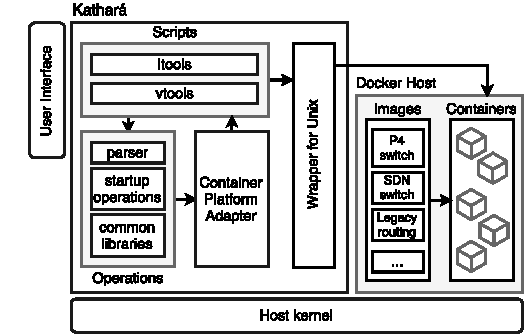
\includegraphics[width=0.8\textwidth]{kathara-architecture-paper}
  \caption{The diagram where Kathara's authors present its architecture}
  \label{fig:kathara-architecture-paper}
\end{figure}


Kathará's own architecture, depicted in figure~\ref{fig:kathara-architecture-paper}, is decribed as comprising three parts:
% Scripts, Operations, and Container Platform Adapter
\begin{description}
  \item[Scripts] used by the users to interact with Kathará.
  These scripts implement the basic operations that are used to start, stop, and pause the network nodes defined in the Kathará configuration and are divided into the two categories referred to in section~\ref{sec:katharafunctionality}, the \texttt{ltools} and the \texttt{vtools}.
  \item[Operations] is a module which \textquote{includes a set of utility functions that are used by the Scripts module in order to allow Kathará to interpret the configuration provided by the users.}
  This module is made of three main logical components: \emph{parser}, \emph{start-up operations}, and \emph{common libraries}.
  The parser is responsible by translating the textual configuration into a network topology; the start-up operations component ensures the cross-system compatibility, namely copying the files that must be copied to inside the nodes;
  \item[Container Platform Adapter] is a layer between the Operations module and Docker, which could allow to use different container platforms other than Docker.
\end{description}

To separate different kinds of nodes with different specific needs in terms of the software (e.g. daemons available to be run) running on them, Kathará allows for its topologies to specify which Docker image it should be running.
The default one (which can be changed on the program's preferences) is \texttt{kathara/quagga}. Therefore, all nodes, are able to launch any of Quagga's functionality, even if they, by omission, don't do it.
For P4 or SDN enabled switches, two different images exist, as well as for the ClickOS-enabled one for creating VNFs.

The Docker networking mechanism~\cite{dockernetworking} to create the collision domains through which interfaces of different containers communicate with each other is not explicitly stated in Kathara's paper.
Therefore, to be sure, one would need to look into the corresponding module on Kathara's source code.

% Kathará also leverages the notion of Docker images, available via Docker Hub or just setup locally on the user's Docker installation, both for separating the functionality (and ``role'') that different kinds of nodes may have on a lab (from being a traditional router to an OpenFlow switch, or an end-host running a RDBMS). % TODO first, take this out of here (maybe to the practical case study, when mentioning the way to create an inherited image), then add RDBMS to the acronyms

% end of section katharatechnicaloverview
